\documentclass[11pt]{beamer}

\usepackage{cedilleverbatim}
\usepackage{times}
\usepackage[absolute,overlay]{textpos}
\usepackage{stmaryrd}
\usepackage{MnSymbol}
\usepackage[normalem]{ulem} %for \sout

\usepackage{tikz}
\usepackage{graphicx}
\usepackage{tabu}
%\usepackage{epstopdf}
\usepackage{color}
%\usepackage{tabularx}
\usepackage{pgflibraryarrows}
\usepackage{pgflibraryshapes}
\usepackage{pgfbaseimage}
\usepackage{listings}

\usetikzlibrary{decorations.text}

%\documentclass{beamer}
%\usepackage{beamerthemesplit}
%\usepackage{mathptmx}
%\usepackage{helvet}

%\usepackage{amsmath}
\usepackage{latexsym}
%\usepackage{amssymb}
\usepackage{proof}
\usepackage{verbatim} 
\usepackage{url}

\definecolor{navy}{RGB}{0,0,128}
\definecolor{dorange}{RGB}{255,100,0}
\definecolor{dgreen}{RGB}{0,75,0}
\definecolor{dbrown}{RGB}{125,30,0}
\definecolor{lbrown}{RGB}{245,150,120}
\definecolor{ored}{RGB}{255,150,70}
\definecolor{oredd}{RGB}{255,69,0}
\definecolor{lightred}{RGB}{255,70,70}
\definecolor{vlred}{RGB}{255,170,170}
\definecolor{cream}{RGB}{255,253,208}
\definecolor{lthistle}{RGB}{185,175,185}

\newcommand{\semeq}[1]{\langle\hspace{-.08cm}|#1|\hspace{-0.08cm}\rangle}
\newcommand{\rep}[1]{\ulcorner #1 \urcorner}
\newcommand{\tlift}[2]{{\uparrow}_{#1}\,(#2)}
\newcommand{\dstar}[0]{\smallstar}
\newcommand{\utp}[0]{\mathcal{U}}
\newcommand{\elcap}[0]{\cap}
\newcommand{\nutt}[4]{\nu\, #1\! :\! #2 \, |\, #3.\, #4}
\newcommand{\interp}[1]{\llbracket #1 \rrbracket} 
\newcommand{\abs}[4]{{#1}\, #2\! : \! #3.\, #4}

% unicode
\usepackage[utf8]{inputenc}
\DeclareUnicodeCharacter{2605}{\ensuremath{\star}}
\DeclareUnicodeCharacter{2081}{\ensuremath{_1}}
\DeclareUnicodeCharacter{2082}{\ensuremath{_2}}
\DeclareUnicodeCharacter{2228}{\ensuremath{\vee}}
\DeclareUnicodeCharacter{27E6}{\ensuremath{\llbracket}}
\DeclareUnicodeCharacter{27E7}{\ensuremath{\rrbracket}}
\DeclareUnicodeCharacter{228E}{\ensuremath{\uplus}}
\DeclareUnicodeCharacter{2113}{\ensuremath{\ell}}
\DeclareUnicodeCharacter{2294}{\ensuremath{\sqcup}}
\DeclareUnicodeCharacter{2192}{\ensuremath{\to}}
\DeclareUnicodeCharacter{2200}{\ensuremath{\forall}}
\DeclareUnicodeCharacter{22CE}{\ensuremath{\curlyvee}}
\DeclareUnicodeCharacter{2115}{\ensuremath{\mathbb{N}}}
\DeclareUnicodeCharacter{2238}{\ensuremath{\dotdiv}}
\DeclareUnicodeCharacter{2261}{\ensuremath{\equiv}}
\DeclareUnicodeCharacter{3BB}{\ensuremath{\lambda}}
\DeclareUnicodeCharacter{1D539}{\ensuremath{\mathbb{B}}}
\DeclareUnicodeCharacter{1D543}{\ensuremath{\mathbb{L}}}
\DeclareUnicodeCharacter{1D54A}{\ensuremath{\mathbb{S}}}
\DeclareUnicodeCharacter{1D54B}{\ensuremath{\mathbb{T}}}
\DeclareUnicodeCharacter{1D54D}{\ensuremath{\mathbb{V}}}
\DeclareUnicodeCharacter{D7}{\ensuremath{\times}}
\DeclareUnicodeCharacter{25C2}{\ensuremath{:}}

\newcommand{\myb}[0]{\ensuremath{\textcolor{blue}{\triangleright}}}

\newcommand{\fore}[0]{\ensuremath{F_\omega^{\textit{rec}}}}

\mathchardef\mhyph="2D % Define a "math hyphen"

\mode<presentation>
{
  %\usetheme{Warsaw}
  % or ...

%\usetheme{IowaCity}
\usetheme{Boston}
%\usetheme{Savannah}

%  \setbeamercovered{transparent}
  % or whatever (possibly just delete it)
}

\usepackage[english]{babel}
% or whatever

\usepackage{times}
\usepackage[T1]{fontenc}
% Or whatever. Note that the encoding and the font should match. If T1
% does not look nice, try deleting the line with the fontenc.



\date{\ }

\begin{document}


\setbeamercolor{normal text}{bg=white,fg=black}

\begin{frame}
\begin{center}
  \Huge
  Lab

  \vspace{1cm}


  

  \end{center}

\end{frame}

\begin{frame}
\begin{center}
  \Huge

\includegraphics[width=4cm]{cedillespiral}

  \vspace{1cm}


  \textcolor{red}{Future directions}

  \end{center}

\end{frame}

\begin{frame}
  \frametitle{Roadmap}

\begin{center}
  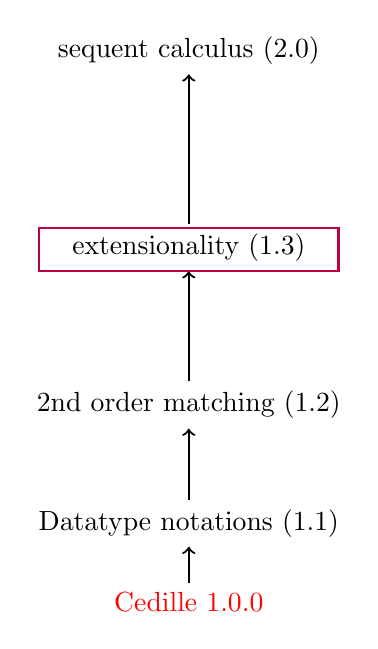
\begin{tikzpicture}

    \node at (0,-1)(v) {\textcolor{red}{Cedille 1.0.0}};

    \pause

    \node at (0,0)(a) {Datatype notations (1.1)};

    \draw[->,thick] (v) -- (a);

    \pause

    \node at (0,1.5)(b) {2nd order matching (1.2)};

    \draw[->,thick] (a) -- (b);

    \pause

    \node at (0,3.5)(c) {extensionality (1.3)};

    \draw[->,thick] (b) -- (c);

    \pause

    \node at (0,6)(d) {sequent calculus (2.0)};

    \draw[->,thick] (c) -- (d);

    \pause

    \draw[thick,purple] (-1.9,3.75) rectangle (1.9,3.2);

%    \draw[thick,purple] (-2.1,6.25) rectangle (2.1,5.7);


  \end{tikzpicture}
\end{center}

  \end{frame}
        
\begin{frame}
  \frametitle{Datatype notations (Cedille 1.1)}

  \begin{itemize}
  \item[$\myb$] High-level notation (like Coq/Agda) for
    \begin{itemize}
    \item Declaring datatypes
    \item Pattern-matching recursion
    \end{itemize}
\vspace{.18cm}
  \item[$\myb$] Elaboration to pure lambda calculus!
\vspace{.2cm}
  \item[$\myb$] The theory we have supports
    \begin{itemize}
    \item Provably monotone datatypes
    \item Histomorphic recursion
    \end{itemize}
  \end{itemize}
\end{frame}

\begin{frame}
  \frametitle{Seeking extensionality}

\Large

  \[
  \begin{array}{c}
    \forall\ x : A.\ \{ f\ x \simeq g\ x \}
    \\    \\
    \Downarrow
    \\    \\
    \{ f \simeq g \}
  \end{array}
  \]

  \end{frame}

\newcommand{\csimeq}[1]{\simeq_{\color{red}#1}}

\begin{frame}
  \frametitle{In extensional MLTT}

\Large

  \[
  \begin{array}{c}
    \forall\ x : A.\ \{ f\ x \csimeq{B} g\ x\}
    \\    
    \Downarrow
    \\    
    x : A \vdash \{ f\ x \csimeq{B} g\ x \}
    \\
    \Downarrow
    \\    
    \{ \lambda\, x.\, f\ x \csimeq{A\to B} \lambda\, x.\, g\ x \}
    \\
    \Downarrow
    \\    
    \{ f \csimeq{A\to B} g \}
  \end{array}
  \]

  \vspace{1cm}

\pause
  \begin{center}
\color{purple}
\Large
    \fbox{Seems to require typed equality!}
    \end{center}

  \end{frame}

\begin{frame}
  \frametitle{Extending Cedille's equality}

  \begin{itemize}
    \item[$\myb$]
  Currently:
  \[
  \begin{array}{c}
    \{ t \simeq t'\} \\ \\
    \interp{\{ t \simeq t'\}} \ \ = \ \ \{ \hat{t}\ |\ \interp{t} =_{\beta\eta} \interp{t'} \}
    \end{array}
  \]

    \item[$\myb$]
  Proposed:
  \[
  \begin{array}{lcl}
    \multicolumn{3}{c}{\{ t \simeq t'\ @\ T\}} \\ \\
    \interp{\{ t \simeq t'\ @\ T\}} & = & \textit{Eq}_{T}\ t\ t' \\
    \textit{Eq}_{A\to B}\ t\ t' & \Leftrightarrow & \forall\ t_1\in\interp{A}.\ \textit{Eq}_{B}\ (t\ t_1)\ (t'\ t_1)\\
    \multicolumn{3}{l}{\cdots}
    \end{array}
    \]


\vspace{.5cm}

      \large\color{purple}
      \fbox{Terms equal at $T$ iff indistinguishable by $T$-contexts}

    
    \end{itemize}

\end{frame}

\begin{frame}
  \frametitle{This is not ETT}

  \underline{In ETT:}

  \[
  \infer{\Gamma\vdash t =_A t' : \star}{\Gamma\vdash t : A \qquad \Gamma\vdash t' : A}
  \]

\vspace{1cm}

  \underline{In proposed extension:}
  
  \[
  \infer{\Gamma\vdash \{ t \simeq t'\ @\ T \} : \star}{\Gamma\vdash T: \star \qquad \textit{FV}(t\ t')\subseteq\textit{dom}(\Gamma)}
  \]

  \end{frame}

\begin{frame}
  \frametitle{(Strange) Example}

  \[
  \textit{True}\ \ =\ \ \forall\ X:\star.\ X \to X
  \]

  The following are equal at type $\textit{True}\to\textit{True}$:
  \[
  \begin{array}{l}
    \lambda\,s.\,\lambda\,z.\, s\ (s\ (z\ \lambda\, q.\,q))\\ \\
    \lambda\,s.\,\lambda\,z.\, s\ (z\ \lambda\, q.\,q)
  \end{array}
  \]

  \begin{itemize}
  \item[$\myb$] Neither term has type $\textit{True}\to\textit{True}$
  \item[$\myb$] Applied to $\lambda\,x.\,x$, they are $\beta$-equal
  \end{itemize}
\end{frame}

\begin{frame}
  \frametitle{Why?}

  \begin{itemize}
  \item[$\myb$] General considerations, and

\vspace{1cm}

  \item[$\myb$] Certain examples, including higher-order abstract syntax

    \[
    \textit{LamTrm}\ : \ \star \ \ = \ \ \forall\ X:\star.((X \to X) \to X) \to (X \to X \to X) \to X
    \]
    \end{itemize}
\end{frame}

\begin{frame}
  \frametitle{Sequent calculus?}

  \begin{itemize}
  \item[$\myb$] Good formalism for duality

\vspace{.2cm}

\item[$\myb$] Under CH, supports control

  \vspace{.2cm}

\item[$\myb$] Challenge: retain canonicity

  \begin{itemize}
  \item BiInt adds dual to subtraction, loses disjunction property
  \item With T. Cantor: logic $\textbf{2Int}^{x}$
  \end{itemize}

  \vspace{.2cm}

  \item[$\myb$] Motivation: coinduction dual to induction
\end{itemize}

\end{frame}

\newcommand{\qlogo}[1]{\raisebox{-.25\height}{
\includegraphics[width=#1]{logo}}?}

\newenvironment{planslide}[2]{%
\begin{frame}
\frametitle{#2}

\large 

\begin{tabular}{l c l }

\qlogo{.7cm} &\ & \textcolor{#1}{Motivation and background for Cedille} \\ \\


$\vdash \textit{\textcolor{red}{C}e\textcolor{red}{D}i\textcolor{red}{L}l\textcolor{red}{E}}$ &\ & \textcolor{#1}{Syntax and semantics}\\ \\

\texttt{cedille} &\ & \textcolor{#1}{Tooling: emacs frontend $\leftrightarrow$ backend} \\ \\

$\leadsto\ \texttt{cedille}_{\texttt{core}}$ & \ & \textcolor{#1}{Elaboration to Cedille Core} \\ \\

\texttt{c d ll} &\ & \textcolor{#1}{Spine-local type inference} \\ \\ 

%\begin{tikzpicture}[
%  decoration={
%    reverse path,
%    text effects along path,
%    text={cedille cedille cedille cedille cedille cedille cedille cedille cedille cedille cedille cedille cedille cedille
%      cedille cedille cedille cedille cedille cedille cedille cedille cedille.},
%    text effects/.cd,
%      text along path,
%      character count=\i, character total=\n,
%      characters={scale=1-\i/\n}
%    }
%]
%\draw [decorate] (0,0) 
%    \foreach \i [evaluate={\r=(\i/2400)^2;}] in {0,7,...,2380}{ -- (\i:\r)}; 
%\end{tikzpicture}

\raisebox{-.8\height}{
\includegraphics[width=2cm]{cedillespiral}} &\ & 

\textcolor{#1}{Future directions}


\end{tabular}

\end{frame}
}



\planslide{red}{Recap}


\begin{frame}
  \frametitle{Thanks}


  Rest of Cedille dev:
  
  \hspace{1cm} Anthony Cantor, Larry Diehl, Andrew Marmaduke

\vspace{1cm}

  Denis Firsov

\vspace{1cm}

  U. Iowa Computational Logic Center (Tinelli, Chowdhury, Reynolds)

\vspace{1cm}

  Funders: NSF, AFOSR(MURI)

\end{frame}


\begin{frame}
\begin{center}

\vspace{1cm}


\includegraphics[width=4cm]{logo}
\end{center}
\end{frame}

\end{document}
